\documentclass[11pt,a4paper]{article}

%==============================================================================%

\usepackage{a4wide}
\usepackage{amsmath,amssymb}
\usepackage[utf8]{inputenc}
\usepackage{float}
\usepackage{graphicx}
\usepackage{listings}
\usepackage{multicol}
\usepackage{tikz}

\usetikzlibrary{arrows}

%==============================================================================%

\newcommand{\assignmentnumber}{2}
\newcommand{\modulus}[1]{\lvert#1\rvert}
\newcommand{\conjugate}[1]{\bar{#1}}
\newcommand{\degree}{^{\circ}}
\newcommand{\limit}[2]{\lim_{#1 \rightarrow #2}}

\newcommand{\figref}[1]{fig. \ref{fig:#1}}
\newcommand{\eqnref}[1]{(\ref{eqn:#1})}

\DeclareMathOperator{\re}{Re}
\DeclareMathOperator{\im}{Im}

\renewcommand\thesection{\assignmentnumber.\arabic{section}}
\renewcommand\thesubsection{\alph{subsection})}

%==============================================================================%

\title{MatIntro Pointopgave \assignmentnumber}
\author
{
    Casper B. Hansen\\
    University of Copenhagen\\
    {\tt fvx507@alumni.ku.dk}
}
\date{\today}

%==============================================================================%

\begin{document}

% \maketitle


% 2.1
\section
{
    \mdseries
    Regn TLO 3.4.12 uden brug af elektroniske hjælpemidler. Vis på en (gerne
    håndtegnet) skitse, hvordan løsningerne ligger i den komplekse plan.
    \\\indent
    Find de komplekse løsninger til ligningen $z^2 - 2iz - (1 + i) = 0$.
    Skriv svaret på formen $a + bi$.
}
Jvf. sætning 3.4.5[TL] har vi, at
\begin{align}
    z &= \frac{-b \pm \sqrt{b^2 - 4ac}}{2a}
       = \frac{-(-2i) \pm \sqrt{(-2i)^2 - 4 \cdot 1 \cdot (1 + i)}}{2 \cdot 1}
       = i \pm \frac{\sqrt{(-2i)^2 - (4 + 4i)}}{2} \\
      &= i \pm \frac{1}{2} \sqrt{(-8 - 4i)}
       = i \pm \frac{1}{2} 2 \sqrt{(-2 - i)}
       = i \pm \sqrt{(-2 - i)}
       \label{eqn:complex-square}
\end{align}
Vi skal nu finde kvadratroden til $(-2 - i)$. Vi bestemme da først modulus;
\begin{align}
    \modulus{(-2 - i)} &= \sqrt{(-2)^2 + (-1)^2}
                        = \sqrt{4 + 1}
                        = \sqrt{5}
\end{align}
Til bestemmelse af argumentet har vi, at
\begin{align}
    \cos \theta = \frac{-2}{\sqrt{5}}
    \qquad
    \sin \theta = \frac{-1}{\sqrt{5}}
    \qquad
    \tan \theta = \frac{\sin \theta}{\cos \theta}
                = \frac{-1 / \sqrt{5}}{-2 / \sqrt{5}}
                = \frac{-1}{-2}
                = \frac{1}{2}
\end{align}
Vi har da, at
\begin{align}
    \sqrt{(-2 - i)}
    &= \sqrt{5} e^{\arctan(\frac{1}{2}) i}
     = \sqrt{5} \left(
        \cos \left( \arctan \left( \frac{1}{2} \right) \right)
        + i \sin \left( \arctan \left( \frac{1}{2} \right) \right) \right) \\
   &= \sqrt{5} \left( \frac{1}{\sqrt{1 + \frac{1}{2}^2}}
   + i \frac{ \frac{1}{2} }{\sqrt{1 + \frac{1}{2}^2}}\right)
    = \sqrt{5} \left( \frac{1 + i \frac{1}{2}}{\sqrt{1 + \left( \frac{1}{2} \right)^2}} \right)
    = \sqrt{5} \left( \frac{1 + i \frac{1}{2}}{\sqrt{5 \left( \frac{1}{2} \right)^2 }} \right) \\
   &= \sqrt{5} \left( \frac{1 + i \frac{1}{2}}{\frac{1}{2} \sqrt{5}} \right)
    = \frac{1 \sqrt{5} + i \frac{1}{2} \sqrt{5}}{\frac{1}{2} \sqrt{5}}
    = \frac{1 + i \frac{1}{2}}{\frac{1}{2}}
    = 2 + i
\end{align}

\begin{multicols*}{2}
    Vi fortsætter da vores udregning fra \eqnref{complex-square}, ved at
    erstatte $\sqrt{(-2 - i)}$ med den beregnede $2 + i$, og får løsningerne
    \begin{align*}
        z_1 &= i + (2 + i) = 2 + 2i \\
        z_2 &= i - (2 + i) = -2
    \end{align*}
    
    Som illustreret i \figref{z1&z2} til højre, er $z_1$ et komplekst tal,
    hvorimod $z_2$ er et reelt talt, da det ikke har nogen imaginær komposant.

    \vfill{\ }\columnbreak

    \begin{figure}[H]
        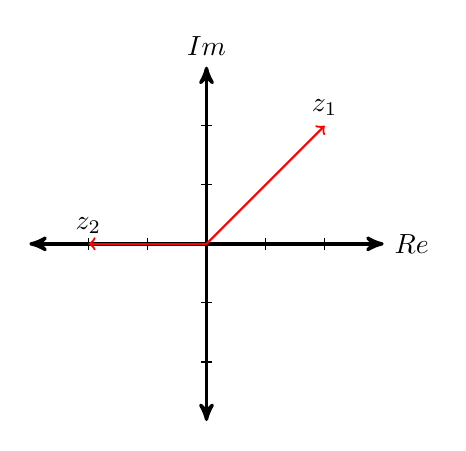
\begin{tikzpicture}[
            scale=0.75,
            axis/.style={very thick, <->, >=stealth'},
            vector/.style={thick, ->,color=red},
            important line/.style={thick},
            dashed line/.style={dashed, thin},
            pile/.style={thick, ->, >=stealth', shorten <=2pt, shorten
            >=2pt},
            every node/.style={color=black}
            ]
            % axis
            \draw[axis] (-3,0)  -- (3,0) node(xline)[right]{$Re$};
            \draw[axis] (0,-3) -- (0,3) node(yline)[above]{$Im$};

            \draw (-2.0, -0.1) -- (-2.0, 0.1);
            \draw (-1.0, -0.1) -- (-1.0, 0.1);
            \draw ( 1.0, -0.1) -- ( 1.0, 0.1);
            \draw ( 2.0, -0.1) -- ( 2.0, 0.1);

            \draw (-0.1, -2.0) -- (0.1, -2.0);
            \draw (-0.1, -1.0) -- (0.1, -1.0);
            \draw (-0.1,  1.0) -- (0.1,  1.0);
            \draw (-0.1,  2.0) -- (0.1,  2.0);

            \draw[vector] (0.0, 0.0) -- ( 2.0, 2.0) node(z1)[above]{$z_1$};
            \draw[vector] (0.0, 0.0) -- (-2.0, 0.0) node(z2)[above]{$z_2$};

        \end{tikzpicture}
        \caption{Illustration af løsningerne $z_1$ og $z_2$ i den komplekse plan}
        \label{fig:z1&z2}
    \end{figure}
\end{multicols*}

% 2.2
\clearpage
\section
{
    \mdseries
    Betragt funktionen $f(x) = \frac{2x^2 - x - 1}{x^2 + 3x + 2}$, $x \in
    [0,\infty[$.
}
I det følgende vil jeg benævne $P(x) = 2x^2 - x - 1$ og
$Q(x) = x^2 + 3x + 2$, for $x \in [0,\infty[$.

\subsection{\mdseries Tegn funktionens graf med Maple.}
\begin{multicols}{2}
    \begin{figure}[H]
        \label{fig:2.2-a}
        \includegraphics[scale=0.5]{figures/2-2a-fig-1.png}
        \caption{Graf for $f$ i $x \in [0,100]$}
    \end{figure}
    \vfill\columnbreak
    \begin{figure}[H]
        \label{fig:2.2b}
        \includegraphics[scale=0.5]{figures/2-2b-fig-1.png}
        \caption{Graf for $f'$ i $x \in [0,100]$}
    \end{figure}
\end{multicols}

\subsection{\mdseries Udregn den afledede $f'(x)$ (benyt gerne Maple) og vis,
    at den er positiv for alle $x \in [0,\infty[$.}
\begin{align}
    f'(x) &= \left( \frac{P(x)}{Q(x)} \right)'
           = \frac{P(x)' Q(x) - P(x) Q(x)'}{Q(x)^2} \\
          &= \frac{(4x - 1)(x^2 + 3x + 2) - (2x^2 - x - 1)(2x + 3)}
                  {(x^2 + 3x + 2)^2} \\
          &= \frac{7x^2 + 10x + 1}{(x^2 + 3x + 2)^2}
           = (7x^2 + 10x + 1) Q(x)^{-2}
           \label{eqn:f'}
\end{align}

En måde, at vise $f'$ er positiv i intervallet $[0,\infty[$ er, at bemærke at
begge andengradspolynomierne $7x^2 + 10x + 1$ hhv. $x^2 + 3x + 2$ består
udelukkende af positive koefficienter. Vi ser bla., at deres skæring med
andenaksen er $c = 1$ hhv. $c = 2$. Ydermere, så er deres afledte funktioners
skæring med andenaksen $b = 10$ hhv. $b = 3$. Det fremgår af $(ax^2 + bx + c)'
= 2ax + b$. Hvilket betyder at tilvæksten for begge må nødvendigvis være
positiv i $x = 0$. Sidst, men ikke mindst, så ved vi, at andengradspolynomier
har et og kun ét lokalt ekstremum, og når $a > 0$ er parablen konveks og
derfor er dette ekstremum et lokalt minimum. Når vi nu ved, at deres afledte
har positiv tilvækst i $x = 0$, må tangenten i dette punkt nødvendigvis
tilhøre højresiden af parablen --- hvilket jo så medfører, at tangenten vokser
når $x \rightarrow \infty$.

En mere koncis måde, kunne være at påvise at $f'$ har kun negative rødder;
$-\frac{5}{7} + \frac{3}{7} \sqrt{2}$ hhv. $-\frac{5}{7} - \frac{3}{7}
\sqrt{2}$, og da $f'(0) = \frac{1}{4}$ følger det, at $f'(x) > 0$, $\forall x
\in [0,\infty[$.

\subsection{\mdseries Bestem $\lim_{n \rightarrow \infty}f(n)$ (benyt ikke
    Maple).}
Det fremgår tydeligt af grafen til $f$ at funktionen har asymptote i $y = 2$

Hvis vi først og fremmest dividere $P(x)$ med dets højeste potensled $x^2$,
kan vi nemmere bestemme grænseværdien for $f$. Så vi har at
\begin{align}
    \frac{2x^2 - x - 1}{x^2 + 3x + 2} &= \frac{2 - 1/x - 1/x^2}{1 + 3/x + 2/x^2}
\end{align}

Vi bemærker, at alle led hvori $x$ indgår nu er på formen $\frac{k}{x^a}$,
og siden $\limit{x}{\infty} k \frac{1}{x^a} = k \cdot \left( \limit{x}{\infty}
\frac{1}{x} \right)^a$, samt reglen om at $\limit{x}{\infty} f(x) + g(x) =
\limit{x}{\infty} f(x) + \limit{x}{\infty} g(x)$ og vi ved at
$\limit{x}{\infty} \frac{1}{x} = 0$, har vi, at samtlige af disse led bliver
nul. Derfor må
\begin{align}
    \limit{x}{\infty}
    \frac{2 - 1/x - 1/x^2}{1 + 3/x + 2/x^2} &= \frac{2}{1} = 2
    \quad
    \text{\textnormal altså er}
    \quad
    \limit{n}{\infty} f(n) = 2
\end{align}

\subsection{\mdseries Bestem værdimængden for $f$.}
Den øvre grænse $\limit{x}{\infty} f(x) = 2$ er allerede fundet. Idet vi har
påvist, at $f'(x) > 0$, $\forall x \in [0, \infty[$ ved vi, at $f$ vil være
voksende i hele definitionsmængden, og finder da nemt den nedre grænse for
$f$ ved indsættelse af laveste $x$-værdi;
\begin{align}
    f(0) &= \frac{2 \cdot 0^2 - 0 - 1}{0^2 + 3 \cdot 0 + 2}
          = -\frac{1}{2}
\end{align}

Altså er værdimængden $V_f = [-0.5,2[$. Bemærk, at den øvre grænse ikke er
med i værdimængden, da funktionen er asymptote i $y = 2$.

\subsection{\mdseries Lad $\epsilon = 0.1$. Bestem en værdi af $N$, som kan
    anvendes i TL definition 4.3.1, når denne definition benyttes på
    grænseovergangen i (c). Du må gerne benytte Maple til at finde en værdi
    af $N$, men du skal argumentere for, at den faktisk kan anvendes. Gentag
    for $\epsilon = 0.01$.}
Først beregner vi $\modulus{a_n - a}$
\begin{align}
    |a_n - a| &= \left| \frac{2n^2 - n - 1}{n^2 + 3n + 2} - 2 \right|
               = \left| \frac{2n^2 - n - 1}{n^2 + 3n + 2} - 2
                        \frac{n^2 + 3n + 2}{n^2 + 3n + 2} \right| \\
              &= \left| \frac{2n^2 - n - 1 - 2(n^2 + 3n + 2)}
                             {n^2 + 3n + 2} \right| \\
              &= \left| \frac{2n^2 - n - 1 - 2n^2 - 6n - 4}
                             {n^2 + 3n + 2} \right|
               = \left| \frac{-7n - 5}{n^2 + 3n + 2} \right| \\
              &= \frac{7n + 5}{n^2 + 3n + 2}
\end{align}
Da vi nu kender $\modulus{a_n - a}$ skal vi finde en passende værdi af $N$,
således at $\frac{7n + 5}{n^2 + 3n + 2} < \epsilon$

\iffalse

\begin{align}
    \modulus{a_n - a} = \frac{7n + 5}{n^2 + 3n + 2} < \epsilon \implies
    \frac{n^2 + 3n + 2}{7n + 5} &> \epsilon^{-1} \\
    n^2 + 2n + 2 &> (7n + 5) \epsilon^{-1} \\
    \epsilon(n^2 + 2n + 2) &> 7n + 5 \\
    \epsilon n^2 + \epsilon 2n + \epsilon 2) &> 7n + 5 \\
\end{align}
Hvis vi dividerer polynomierne vha. $\frac{P(x)}{Q(x)} = K(x) +
\frac{R(x)}{Q(x)}$ har vi, at
\begin{align}
    \frac{n^2 + 3n + 2}{7n + 5}
    &= \frac{n}{7} + \frac{16}{49} + \frac{18 / 49}{(7n + 5)}
\end{align}

Hvis vi dividerer polynomierne vha. $P(x) = K(x) Q(x) + R(x)$ har vi, at
\begin{align}
    n^2 + 3n + 2 &= \left( \frac{n}{7} + \frac{16}{49} \right)
                    \left( 7n + 5 \right)
                  + \frac{18}{49}
\end{align}

\fi

Jeg benytter mig af Maple til, at finde disse værdier, og får at
\begin{align}
    N_1 = 67.70891697 \text{, for } \epsilon_1 = 0.1
    \qquad
    \text{og}
    \qquad
    N_2 = 697.7137598 \text{, for } \epsilon_2 = 0.01
\end{align}

Vi bemærker, at $\limit{n}{\infty} \modulus{a_n - a} = 0$. Dvs. udtrykket
går altså imod nul som $n$ bevæger sig mod $\infty$, og $0 < \epsilon_2 <
\epsilon_1$. Derfor holder
\begin{align}
    \modulus{a_n - a} &= \frac{7n + 5}{n^2 + 3n + 2} < \epsilon_1
    \text{, hvis og kun hvis } n > N_1 \\
    \modulus{a_n - a} &= \frac{7n + 5}{n^2 + 3n + 2} < \epsilon_2
    \text{, hvis og kun hvis } n > N_2
\end{align}

% 2.3(iv)
\section
{
    \mdseries
    Denne opgave omhandler, hvor hurtigt kaniner kan formere sig under
    idealiserede forhold. Vi antager, at vi starter med par nyfødte kaniner,
    en han- og en hunkanin. Forestil dig, at kaniner kan formere sig, når de
    er 1 måned gamle, og en hunkanin har en drægtighedsperiode på 1 måned, så
    ved udgangen af den 2. måned kan hun-kaninen føde et nyt kaninpar (men det
    nye kuld kommer først til umiddelbart efter 2. måned, således at der i 2.
    måned stadig kun er 1 kaninpar.) Vi antager, at vores kaniner ikke dør,
    og der ved hver fødsel kommer et kaninpar bestående af en han- og en
    hunkanin.
    \\\indent
    Lad $n \in \mathbb{N}$ betegne måned nummer $n$, med $n=1$ som den
    første måned. Lad $F_n$ betegne antallet af kaninpar i måneden $n$. Hvis
    kaninerne får lov til at formere sig til frit, vil det samlede antal
    kaninpar være summen af par de to foregående måned.
}
\begin{align}
    F_{n+2} = F_n + F_{n+1}
\end{align}

\subsection
{
    \mdseries
    Giv en intuitiv forklaring på denne rekursionsformel. Hvad er
    begyndelsesbetingelserne $F_1$, $F_2$ i vores tilfælde? Bestem, hvor
    mange kaninpar der således vil være efter 1 år.
}
I første måned har vi det nyfødte kaninpar, og dermed er $F_1 = 1$. Ved
begyndelsen af anden måned antages hunkaninen, at være drægtig, og siden en
drægtighedsperioden er en måned, så må $F_2 = 1$ også. Det er altså først i
tredje måned, hvor det første kuld fødes.
\begin{align}
    F_1 = 1
    \qquad
    F_2 = 1
\end{align}
I ord, kan man sige at $F_{n+2}$ er antallet af kaninpar, som under disse
ideelle omstændigheder, kan produceres af den foregående generation $F_n$,
samt den nye generation $F_{n+1}$.

Til bestemmelse af antal kaninpar, med disse startbetingelser, efter 1 år,
har vi at
\begin{align}
    F_{12} &= F_{10} + F_{11} \\
           &= F_8 + 2 F_9 + F_{10} \\
           &= F_6 + 3 F_7 + 3 F_8 + F_9 \\
           &= F_4 + 4 F_5 + 6 F_6 + 4 F_7 + F_8 \\
           &= F_2 + 5 F_3 + 10 F_4 + 10 F_5 + 5 F_6 + F_7 \\
           &\vdots \\
           &= 144 F_1 = 144
\end{align}

Bemærk, at koefficienterne i lignerne ovenfor følger Pascal's trekant.

\subsection
{
    \mdseries
    Vis at elementerne i følgen ${F_n}$ opfylder $F_n \leq F_{n+1} \leq 2F_n$
    for ethvert $n \in \mathbb{N}$.
    \\\indent
    Vi definerer vækstraten for kaninbestanden ved $a_n =
    \frac{F_{n+1}}{F_n}$. Udregn vækstraten for $n = 1, 2, \dots, 12$ og
    illustrer de beregnede værdier af $a_n$ ved brug Maple.
}
Vi viser først, at $F_n$ opfylder uligheden for $n=1$
\begin{align}
    F_1 \leq F_{1+1} \leq 2F_1 &= 1 \leq 1 \leq 2
\end{align}
Dernæst viser vi, at $F_n$ opfylder uligheden for $n=k$, hvor $k \in
\mathbb{N}$, altså
\begin{align}
    F_k \leq F_{k+1} \leq 2F_k
    &\implies
    F_{k-2} + F_{k-1} \leq F_{k-1} + F_{k} \leq 2F_{k-2} + 2F_{k-1} \\
    &\implies
    F_{k-2} \leq F_{k} \leq 2F_{k-2} + F_{k-1} \\
    &\implies
    0 \leq F_{k} - F_{k-2} \leq F_{k-2} + F_{k-1} \\
    &\implies
    0 \leq F_{k} - F_{k-2} \leq F_{k}
\end{align}
Det er tydeligt at se, at $F_n$ opfylder uligheden idet $0 \leq k - a \leq k$,
$\forall k, a \in \mathbb{N}$.

\begin{multicols}{2}
    \begin{figure}[H]
        \includegraphics[scale=0.5]{figures/2-3b-fig-1.png}
        \caption{Grafen for $F_n$ i $n \in [1,12]$}
        \label{fig:2.3b-1}
    \end{figure}
    \vfill\columnbreak
    \begin{figure}[H]
        \includegraphics[scale=0.5]{figures/2-3b-fig-2.png}
        \caption{Grafen for $a_n$ i $n \in [1,12]$}
        \label{fig:2.3b-2}
    \end{figure}
\end{multicols}

\subsection
{
    \mdseries
    Anfør ud fra din illustration i (b) et træk ved den første del af følgen
    ${a_n}$, der taler for, at følgen konvergent. Vi tillader os nu at
    antage, at dette kan uddybes til et bevis for at følgen {\it er}
    konvergent.
    \\\indent
    Bestem grænseværdien, $a$, af $a_n$ for $n \rightarrow \infty$ uden brug
    af Maple. [Vink: opstil først rekursionsformlen $a_{n+1} = 1 +
    \frac{1}{a_n}$ ud fra (1) og se, hvad der sker når $n \rightarrow
    \infty$.]
}
Det lader til, at $F_{2n - 1} < k < F_{2n}$, $\forall n \in \mathbb{N}$, og
$a_{n+1} < a_n$. Med andre ord, $F_n < a_n$, hvis $n$ er ulige og omvendt er
$F_n > a_n$, hvis $n$ er lige. Dermed, så må $a_n$ konvergere mod $k$.

Det ses også tydeligt på grafen for $a_n$ i \figref{2.3b-2}, at forholdet
mellem $F_{n+1}$ og $F_n$ konvergerer mod et tal $k$.

Vi opstiller forholdet, og beregner
\begin{align}
    a_n &= \frac{F_{n+1}}{F_n}
         = \frac{F_{n-1} + F_n}{F_n}
         = \frac{F_{n-1}}{F_n} + \frac{F_n}{F_n}
         = 1 + \frac{F_{n-1}}{F_n}
         = 1 + \frac{F_{n-1}}{F_n}
         = 1 + \frac{1}{F_n / F_{n-1}}
         = 1 + \frac{1}{a_{n-1}}
\end{align}

Vi ser nu på, hvad grænseværdien $a = \limit{n}{\infty} \left( 1 +
\frac{1}{a_{n-1}} \right)$
\begin{align}
    \limit{n}{\infty} a_n &= 1 + \frac{1}{\limit{n}{\infty} a_{n-1}}
    \implies a = 1 + \frac{1}{a}
    \implies a^2 = a + 1
    \implies a^2 - a - 1 = 0
\end{align}

Dette er en andengradspolynomium, for hvilket vi kan løse for $a$
\begin{align}
    a &= \frac{-(-1) \pm \sqrt{(-1)^2 - 4 \cdot 1 \cdot (-1)}}{2 \cdot 1}
       = \frac{1 \pm \sqrt{5}}{2}
\end{align}

\subsection
{
    \mdseries
    Hvis (1) i stedet (under passende begyndelsesbetingelser) havde været
    $F_{n+2} = F_n + F_{n+1} - \alpha$ eller $F_{n+2} = F_n + F_{n+1} -
    \gamma F_{n+1}$, med $\alpha \in \mathbb{N}$ og $\gamma \in ]0,1[$,
    hvad ville modellen så beskrive? Er dette en mere realistisk model?
}
I første tilfælde, hvor $F_{n+2} = F_n + F_{n+1} - \alpha$, hvor $\alpha \in
\mathbb{N}$, beskriver modellen et statisk dødsfald, hver måned, uafhængigt
af kaninbestanden. Denne model er lidt mere realistisk end den oprindelige.

For det andet tilfælde, hvor $F_{n+2} = F_n + F_{n+1} - \gamma F_{n+1}$,
hvor $\gamma \in ]0,1[$, beskriver modellen da et dynamisk procentvis
dødsfald i den forrige generation $F_{n+1}$. Idet $0 < \gamma < 1$ er vi
sikre på, at en hvis procentdel af den forrige generation dør, men aldrig
hele generationen. Antal dødsfald i den forrige generation kan altså
beskrives ved $\gamma F_{n+1}$, eller modsat antal overlevende kan beskrives
ved $(1 - \gamma) F_{n+1}$ og dødsfaldsprocenten kan beskrives ved $1 -
\gamma$ --- ved omformulering af udtrykket har vi da, at $F_{n+2} = F_n + (1
- \gamma) F_{n+1}$. Denne model er nok den mest realistiske, da dødsfaldet
afhænger af bestanden.

\end{document}
